\par
\chapter{{\tt Chv}: Block chevron}
\par
The {\tt Chv} object is used to store and operate on a {\it front}
during a sparse factorization.
The {\tt Chv} object can contain either double precision real or
complex data.
A front is a portion of a matrix, shaded grey in the diagram below.
\begin{center}
\makebox{
% \psfig{file=simple.eps,width=1.0in,height=1.00in}
\psfig{file=../../Chv/doc/simple.eps,width=1.0in,height=1.00in}
}
\end{center}
We use the word ``chevron'' to describe the front, because if you
rotate the figure $45^\circ$ clockwise the shaded region resembles
the chevron insignia of enlisted personnel in the armed forces.
Similar matrices are also known as ``arrowhead'' matrices, but we
have found the ``chevron'' has a simpler abbreviation.
We use the adjective ``block'' to emphasize that the chevron object
may have multiple entries of the diagonal of the matrix.
A ``single'' chevron (which is one way we assemble entries from a
matrix into this data structure) contains a single entry from the
diagonal of the matrix.
\par
The shaded region in the diagram above will normally be sparse,
i.e., many of the entries might be zero.
There are three logical blocks to the {\tt Chv} object:
a nonempty square (1,1) block in the upper left corner,
and (possibly empty) (1,2) and (2,1) blocks in the upper right
and lower left corners.
To conserve space and minimize work on logically zero elements,
we store only rows of the lower part and columns of the upper part
that have (or may have) nonzero elements. 
(Note, a particular row or column may 
have zero elements, but normally there will be nonzeros in each row
and column that we store.)
\par
{\tt Chv} objects come in three types --- symmetric, Hermitian and
nonsymmetric.
When an object is symmetric or Hermitian, we only store the upper
triangle.
There is one limitation, perhaps unnecessary,
that we put on the {\tt Chv} object ---
the number of rows in the (2,1) block and number of columns 
in the (1,2) block are equal.
The {\tt Chv} object is used within the context of a factorization
of a sparse matrix that is assumed to have symmetric structure.
If we ever extend the code to handle a true nonsymmetric structure
factorization (e.g., {\sc umfpack} and {\sc superlu}), then we can
modify the {\tt Chv} object to handle unequal rows and columns.
\par
During a factorization,
a front has to take part in four distinct operations.
\begin{enumerate}
\item
Assemble entries from the original matrix (or matrix pencil). 
(See the {\tt Chv\_addChevron()} method.)
\item
Accumulate updates from descendant fronts.
(See the {\tt Chv\_update\{S,H,N\}()} methods.)
\item
Assemble any postponed data from its children fronts.
(See the {\tt Chv\_assemblePostponedData()} method.)
\item
Compute the factorization of the completely assembled front.
(See the {\tt Chv\_factor()} method.)
\end{enumerate}
\par
The implementor of a front object has a great deal of freedom to
design the underlying data structures. 
We have chosen to store the entries in each single chevron
in contiguous memory --- the first entry of a chevron is in 
the last row of the front, the last entry of a chevron is 
in the last column of the front.
The figure below shows the storage locations for the 
entries --- on the left is a nonsymmetric chevron, on the right is
a symmetric or hermitian chevron.
\begin{center}
\makebox{
% \psfig{file=simple2.eps,width=2.2in,height=1.00in}
\psfig{file=../../Chv/doc/simple2.eps,width=2.2in,height=1.00in}
}
\end{center}
\par
Any storage format has advantages and disadvantages.
\begin{itemize}
\item[{\bf con}]
Moving along the diagonal is a nonconstant stride through memory.
The same holds for moving along a row in the lower part and along a
column in the upper part.
While the strides are nonconstant, they are easily determined,
particularly when starting in the first chevron.
This affects the search methods that look for a pivot in the (1,1)
block, the method that evaluates a pivot, 
the swap methods that swap rows and columns,
and the methods that extract the entries from the chevron to be
stored in the factor matrix.
\item[{{\bf pro}}]
Moving along a row in the upper part and along a column in the
lower part uses a unit stride.
This is useful when performing an update to the remaining part of
the front after a pivot element has been selected.
\item[{\bf pro}]
The assembly of data, be it from the original matrix stored by
chevrons, aggregate update fronts from other processes in a
parallel factorization, or postponed data when pivoting for
stability is used can be done in a straightforward manner.
\end{itemize}
\par
The chevron object exists within the context of a larger global
matrix, and so needs indices to define its rows and columns.
For a symmetric or Hermitian matrix, we only store the column
indices.
For a nonsymmetric matrix, we store the both the row and column 
indices.
This second case may seem unnecessary, since we assume that the
larger global matrix has symmetric structure.
However, during a factorization with pivoting enabled,
a pivot element may be chosen from anywhere in the (1,1) block,
so the row indices and column indices may no longer be identical.
\par
A {\tt Chv} object is inherently a serial, single threaded object,
meaning it is designed so that only one thread or process ``owns''
or operates on a particular {\tt Chv} object.
A {\tt Chv} object is an ``atom'' of communication.
It stores postponed rows and columns to be assembled in a parent
front.
It might have to be written to and read from a file in an
out-of-core implementation.
In a distributed environment, it is communicated between processes.
For these reasons, we designed the object so that its data
(the scalars that describe its dimensions, id and type,
the row and column indices, and its entries) are found in
contiguous storage managed by a {\tt DV} object.
A file operation can be done with a single read or write,
a message can be sent without packing and unpacking data,
or defining a new datatype.
Managing working storage for a number of {\tt Chv} objects
is now simpler.
\par
When the {\tt Chv} object contains double precision {\it complex} data,
it stores and operates on them as double precision entries.
We follow the FORTRAN convention that the real and imaginary part
of a complex number are stored consecutively, the real part first
followed by the imaginary number.
In the above complex nonsymmetric matrix, 
the third diagonal entry is found
at location 38 {\it in terms of the complex numbers}, but its real
and imaginary parts are found in locations 2*38 = 76 and 2*38+1 = 77
of the double precision vector that stores the entries.
Computations are done in a mix of subroutine calls
(see {\tt Utilites/ZV.h}) and by expanding the complex arithmetic
into real arithmetic.
\par
The {\tt Chv} object ``knows'' about the {\tt IV}, {\tt DV} and
{\tt ZV} vector objects (for {\tt int}, {\tt double} and
{\tt double complex} data types),
the {\tt A2} object for dense 2-D arrays,
and the {\tt SubMtx} object for dense or sparse 2-D submatrices.
These {\tt IV}, {\tt DV}, {\tt ZV}, {\tt A2} and {\tt SubMtx} objects
are subordinate to the {\tt Chv} object.
